
\documentclass[12pt, a4paper]{article}
\usepackage{fullpage}
\usepackage{graphicx}
\usepackage{wrapfig}
\usepackage{amsmath}
\usepackage{float}
\usepackage{listings}
\usepackage{lmodern}  % for bold teletype font
\usepackage{xcolor}   % for \textcolor

\definecolor{codegreen}{rgb}{0,0.6,0}
\definecolor{codegray}{rgb}{0.5,0.5,0.5}
\definecolor{codepurple}{rgb}{0.58,0,0.82}
\definecolor{backcolour}{rgb}{0.95,0.95,0.92}

\title{\textbf{EE2703 : Applied Programming Lab \\ End-semester exam}} % Title

\author{Potta Muni Asheesh \\ EE19B048} % Author name

\date{\today} % Date for the report

\begin{document}	
\lstset{
  language=Python,
  backgroundcolor=\color{backcolour},   
  commentstyle=\color{codegreen},
  keywordstyle=\color{magenta},
  numberstyle=\tiny\color{codegray},
  %stringstyle=\color{codepurple},
  basicstyle=\ttfamily,
  breakatwhitespace=false,         
  breaklines=true,                 
  captionpos=b,                    
  keepspaces=true,                 
  numbers=left,                    
  numbersep=5pt,                  
  showspaces=false,                
  showstringspaces=false,
  showtabs=false,                  
  tabsize=2,
  columns=fullflexible,
  frame=single,
  postbreak=\mbox{\textcolor{red}{$\hookrightarrow$}\space},
}	
		
\maketitle % Insert the title, author and date

\section{Introduction}

This problem is about a loop antenna whose length is equal to the wave length $\lambda$ of the radiation.

The loop carries a current given by

\begin{equation*}
I = \frac{4\pi}{\mu_0}\cos(\phi)\exp(j\omega t)
\end{equation*}

where, $\phi$ is the polar angle in cylindrical coordinates. The radius of the loop ($a$) is 10cm which is also equal to $\lambda/2\pi = 1/k = c/\omega$, this implies circumference $2\pi a = \lambda$. For a given current, the magnetic vector potential is given by the integral,

\begin{equation*}
\boldsymbol{A}(\boldsymbol{r}, t) = \frac{\mu_0}{4\pi} \int_C \frac{I(\boldsymbol{r'}, t') d\boldsymbol{r'}}{|\boldsymbol{r} - \boldsymbol{r'}|}
\end{equation*}

where C is the curve of the loop, $\boldsymbol{r'}$ is the position of point on the loop and $t' = t - \frac{|\boldsymbol{r} - \boldsymbol{r'}|}{c}$. And from the magnetic vector potential $\boldsymbol{A}$, the magnetic field $\boldsymbol{B}$ is given as $\boldsymbol{B} = \nabla \times \boldsymbol{A}$

\section{Pseudocode}

In the pseudocode below, the procedure or algorithm to solve the problem is given. The declarations in the pseudocode have been written in english language.

\begin{lstlisting}
X, Y, Z are the x, y and z components of meshgrid of x from -1 to 1, y from -1 to 1 and z from 1 to 1000 indexed i,j,k
x' is x-coordinate of 100 sections of the loop indexed by l.
y' is y-coordinate of 100 sections of the loop indexed by l.
phi' is the polar angle of mid point of the 100 sections of the loop indexed by l.
dx' is x-component of dl'
dy' is y-component of dl'
k is the wave constant

Ax and Ay is initially 0.

for l from 0 to 99
    R = sqrt((X-x'[l])^2 + (Y-y'[l])^2 + Z^2)
    Ax += cos(phi'[l])*exp(-j*k*R)*dx'[l]/R
    Ay += cos(phi'[l])*exp(-j*k*R)*dy'[l]/R

Bz = 0.5*(Ay[1, 0, 1 to 1000] - Ax[0, 1, 1 to 1000] - Ay[-1, 0, 1 to 1000] + Ax[0, -1, 1 to 1000])
\end{lstlisting}

\lstset{
  language=Python,
  backgroundcolor=\color{backcolour},   
  commentstyle=\color{codegreen},
  keywordstyle=\color{magenta},
  numberstyle=\tiny\color{codegray},
  stringstyle=\color{codepurple},
  basicstyle=\ttfamily,
  breakatwhitespace=false,         
  breaklines=true,                 
  captionpos=b,                    
  keepspaces=true,                 
  %numbers=left,                    
  %numbersep=5pt,                  
  showspaces=false,                
  showstringspaces=false,
  showtabs=false,                  
  tabsize=2,
  columns=fullflexible,
  frame=single,
  postbreak=\mbox{\textcolor{red}{$\hookrightarrow$}\space},
}

\section{Current elements in the loop}

Since the loop of wire is in the x-y plane, has a radius of $a = 10$cm and centered at the origin. Each point on the loop ($\vec{r'}$) can be denoted in terms of polar angle $\phi$ as

\begin{equation*}
\vec{r'} = a (\cos(\phi) \hat{x} + \sin(\phi) \hat{y} ); 0 \leq \phi < 2\pi
\end{equation*}

And, the current in the loop at time $t = 0$ is given by,

\begin{equation*}
I(\phi) = \frac{4\pi}{\mu_0}cos(\phi)
\end{equation*}

Consider an element of length $dl' = ad\phi$ on the loop, then in cartesian coordinates, the element length vector is given by,

\begin{equation*}
\vec{dl'} = a d\phi (-\sin(\phi) \hat{x} + \cos(\phi) \hat{y})
\end{equation*} 

For computation, the loop is broken into 100 sections and x and y components of $\vec{r'}$ and $\vec{dl'}$ for these 100 sections are obtained in an array as shown.

\begin{lstlisting}
a = 10; k = 1/a

phi = np.linspace(0, 2*np.pi, 101); phi = phi[:-1]
delta_phi = phi[1]-phi[0]
phi += (phi[1]-phi[0])/2 # Setting the point to middle of the element.

x1, y1 = a*np.cos(phi), a*np.sin(phi) # r' vector components
dx1, dy1 = -a*delta_phi*np.sin(phi), a*delta_phi*np.cos(phi) # dl' vector components
\end{lstlisting}

The x and y components of vector $I \vec{dl'} = \cos(\phi)a d\phi \hat{\phi}$ for the 100 sections is obtained as

\begin{lstlisting}
# x and y components of the current element vector (Idl'), 
# alternating elements are considered for visual comfort.
I_x, I_y = (x1[::2]/a)*(dx1[::2]), (x1[::2]/a)*(dy1[::2])
\end{lstlisting}

Note that, the scaling factor $4\pi/ \mu_0$ is not considered for the plot.

The plot of the current element vectors is shown below

\begin{figure}[H]
\centering
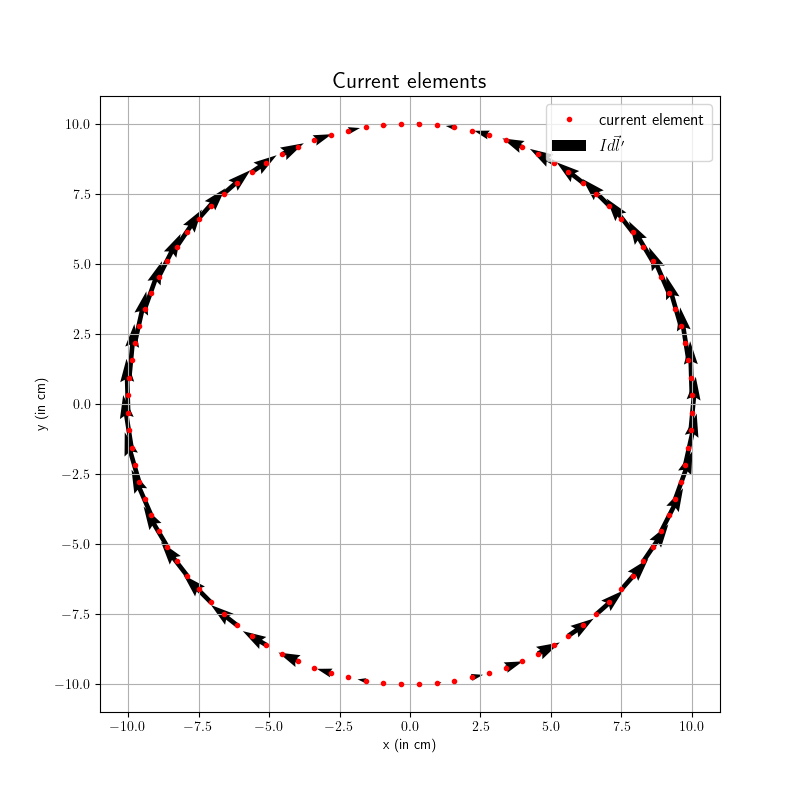
\includegraphics[width=0.8\textwidth]{current.png}
\caption{The vector $I\vec{dl'}$ at each section}
\end{figure}

Note that, alternate vector arrows are shown to avoid clumsiness in the plot.

It can be observed that the current is symmetric about the y-axis. From this, it can be expected that the magnetic field along z-axis ($B_z$) is 0.

\section{Computing the vector potential $\vec{A}$ and magentic field $B_z(z)$}

In order to compute the vector potential, consider a $3 \times 3 \times 1000$ 3D mesh in which x varies from -1cm to 1cm, y varies from -1cm to 1cm and z varies from 1cm to 1000cm. The seperation between each mesh point in a plane is 1cm. It is created as 

\begin{lstlisting}
x = np.linspace(-1.0,1.0,3)  
y = np.linspace(-1.0,1.0,3)
z = np.linspace(1.0, 1000.0, 1000)

X, Y, Z = np.meshgrid(x, y, z, indexing='ij')
\end{lstlisting}

Since, the vector potential $\vec{A_{ijk}}$ is computed numerically as,

\begin{align*}
\left( \vec{A_{ijk}} \right)_x &= \sum_{l = 0}^{99} \frac{\cos(\phi_l)\exp(-jkR_{ijkl})(-\sin(\phi_l))dx'_l}{R_{ijkl}} \\
\left( \vec{A_{ijk}} \right)_y &= \sum_{l = 0}^{99} \frac{\cos(\phi_l)\exp(-jkR_{ijkl})(\cos(\phi_l))dy'_l}{R_{ijkl}}
\end{align*}

where $l$ is the index of the current element and $i, j, k$ are the indices of the points in the mesh $(x_i, y_j, z_k)$, $k = \omega/c$ is the wave propogation constant and $R_{ijkl} = |(x_i - a \cos(\phi_l))\hat{x} + (y_j - a \sin(\phi_l))\hat{y} + (z_k)\hat{z}|$

To compute each term in the summation, a function named \texttt{calc} is defined, which computes and returns both x and y components of the vector potential. It is defined as shown below.

\begin{lstlisting}
def calc(l, x1, y1, dx1, dy1, X, Y, Z, phi, k, dynamic=True):
    """
    This function finds the vector potential due to the current
    element of index l. Here, the current I = (4*pi/mu0)*cos(phi),
    and depending on whether the current is time-dependent or not
    (determined by the boolean parameter 'dynamic'), the current
    is multiplied by exp(j*w*t). Here, first, R = |r - r'| is 
    found and then vector potential A is computed, which has 
    only x and y components.
    """
    Rl = np.sqrt((X-x1[l])**2 + (Y-y1[l])**2 + Z**2)
    if dynamic:
        A_xl = (np.cos(phi[l])*np.exp(-1j*k*Rl)*dx1[l])/Rl
        A_yl = (np.cos(phi[l])*np.exp(-1j*k*Rl)*dy1[l])/Rl
    else:
        A_xl = (np.cos(phi[l])*dx1[l])/Rl
        A_yl = (np.cos(phi[l])*dy1[l])/Rl
    return np.array([A_xl, A_yl])
\end{lstlisting}

Note, the function can be used to compute vector potential for both dynamics and statics, based on the boolean value of the parameter \texttt{dynamic}.

Finally, the summation is done using for loop to iterate over the index $l$. \textit{Vectorized code} could not be used here because a 4 dimensional array cannot be created in any way from a 3 dimensional and a 1 dimensional arrays using math operations.

The summation is done is done as follows,

\begin{lstlisting}
A = calc(0, x1, y1, dx1, dy1, X, Y, Z, phi, k, dynamic=True)
for l in range(1, 100):
    A += calc(l, x1, y1, dx1, dy1, X, Y, Z, phi, k, dynamic=True)
\end{lstlisting}

The magentic field is given by the curl of the vector potential,

\begin{equation*}
\vec{\nabla} \times \vec{A} = \vec{B}
\end{equation*}

The z component of the magnetic field aloong z-axis $B_z(z)$ is given by,

\begin{equation*}
B_z(z) = \frac{\partial A_y}{\partial x} (0,0,z) - \frac{\partial A_x}{\partial y} (0,0,z)
\end{equation*}

Numerically, it computed using the central difference method as 

\begin{equation*}
B_z(z) = \frac{A_y(\Delta x, 0, z) - A_y(-\Delta x, 0, z)}{2\Delta x} - \frac{A_x(0, \Delta y, z) - A_x(0, -\Delta y, z)}{2\Delta y}
\end{equation*}

where, $\Delta x = \Delta y = 1$cm

This is done as shown below.

\begin{lstlisting}
# Finding the curl of the vector potential along the z-axis to find the magentic field.
B_z = np.abs(0.5*(A[1,2,1,:]-A[0,1,2,:]-A[1,0,1,:]+A[0,1,0,:]))
\end{lstlisting}

The logarithmic plot of the z-component of the magnetic field along the z-axis is shown below.

\begin{figure}[H]
\centering
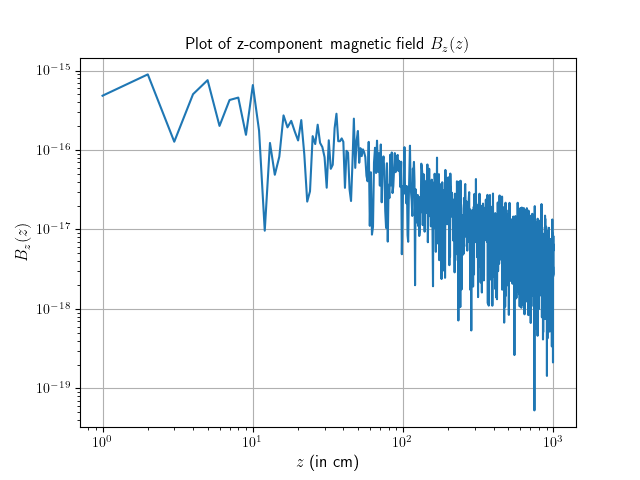
\includegraphics[width=0.8\textwidth]{Bzcos.png}
\caption{The magentic field along the z-axis}
\end{figure}

It can be seen that the magentic field is of the order $10^{-16}-10^{-17}$ which can practical be considered as 0, which is as expected.

\section{Least squares fit}

Consider the model for the magentic field along z-axis to be $B_z = cz^b$, to find a least squares fit for this model, the exponential has to be converted to something linear by taking logarithm, so

\begin{equation*}
\log(B_z) = b \log(z) + \log(c)
\end{equation*}

The corresponding matrix equation is
\begin{equation*}
\left( 
\begin{matrix}
\log(z_0) & 1 \\
\log(z_1) & 1 \\
. & . \\ 
. & . \\
. & . \\
\log(z_{999}) & 1  
\end{matrix}
\right)
\left(
\begin{matrix}
b \\
\log(c)
\end{matrix}
\right) = 
\left( 
\begin{matrix}
\log(B_z(z_0)) \\
\log(B_z(z_1)) \\
. \\ 
. \\
. \\
\log(B_z(z_{999}))
\end{matrix}
\right)
\end{equation*}

The parameters $b$ and $c$ are found as

\begin{lstlisting}
# Finding the least squares fit (b, c) for the model, Bz = c*(z^b)
M = np.c_[np.log(z),np.ones(z.size)]
fit = lstsq(M, np.log(B_z))[0]
b = fit[0]
c = np.exp(fit[1])
print("The approximated values of b and c are {}, {}".format(b, c))
\end{lstlisting}

The plot of the magnetic field given by least squares fit is shown below

\begin{figure}[H]
\centering
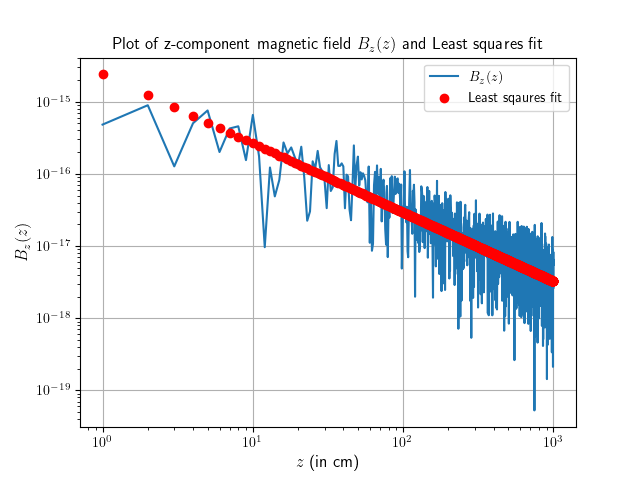
\includegraphics[width=0.8\textwidth]{Bzcosfit.png}
\caption{The magentic field along the z-axis from least squares fit}
\end{figure}

The approximated values of b and c are -0.9558345894653539, 2.3929363959585138e-15

Since the magnetic field is actually 0, the order of the decay of magnetic field can be considered the computational error.

\section{Difference between statics and dynamics}

In the above case, the current changes with time, this is the case of magnetodynamics.

\begin{equation*}
I = I(\phi)\exp(j\omega t)
\end{equation*}

In this case, the vector potential for a given current is given by

\begin{equation*}
\vec{A}(\vec{r}, t) = \frac{\mu_0}{4\pi} \int \frac{I(\phi)\exp(j(\omega t-kR))ad\phi}{R}
\end{equation*}

where, $R = |\vec{r} - \vec{r'}|$, $\vec{r}$ is the point where the vector potential is being caluculated and $\vec{r'}$ is the point on the loop.

Now, consider a current independent of time, say

\begin{equation*}
I = I(\phi)
\end{equation*}

This is the case of magnetostatics. Here, the vector potential is given by

\begin{equation*}
\vec{A}(\vec{r}) = \frac{\mu_0}{4\pi} \int \frac{I(\phi)ad\phi}{R}
\end{equation*}

where, $R$ is same as mentioned above.

Numerically, this becomes,

\begin{align*}
\left( \vec{A_{ijk}} \right)_x &= \frac{\mu_0}{4\pi} \sum_{l = 0}^{99} \frac{I(\phi_l)(-\sin(\phi_l))dx'_l}{R_{ijkl}} \\
\left( \vec{A_{ijk}} \right)_y &= \frac{\mu_0}{4\pi} \sum_{l = 0}^{99} \frac{I(\phi_l)(\cos(\phi_l))dy'_l}{R_{ijkl}}
\end{align*}

For $I(\phi) = \frac{4\pi}{\mu_0} \cos(\phi)$, There is not much difference between dynamics and statics case, both have zero magnetic field along z-axis. 

In order to observe the difference between these two cases, consider $I(\phi) = \frac{4\pi}{\mu_0}$. For this current, in case of magnetostatics, we can analytically find out that magnetic field along z-axis, is given by

\begin{equation*}
B_z(z) = 2\pi \frac{a^2}{(\sqrt{z^2 + a^2})^3}
\end{equation*}

So, the expected decay of the magnetic field is $z^{-3}$. The magnetic field is computed numerically, a function \texttt{calc1} is defined for this (see complete python code given below), and a least squares fit of type $B_z(z) \approx cz^b$ is found, it looks like

\begin{figure}[H]
\centering
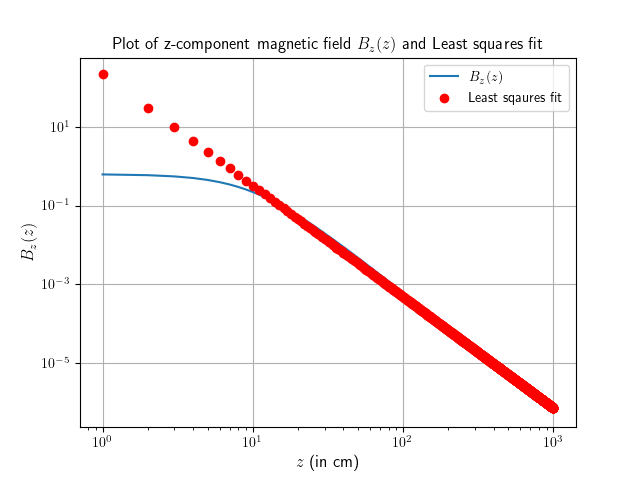
\includegraphics[width=0.75\textwidth]{Bzconstfit.png}
\caption{The magentic field along the z-axis from least squares fit}
\end{figure}

Here, the approximated values of b and c are -2.8261920569266086, 215.85790244337815, which is very near to the analytical value of b = -3.

For the magnetodynamics case, find the analytical answer is difficult. So, directly the numerical answer is computed at time $t = 0$ and it is obtained as,

\begin{figure}[H]
\centering
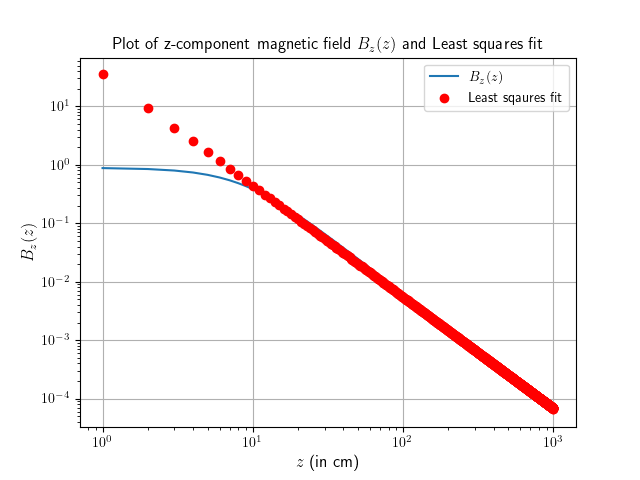
\includegraphics[width=0.75\textwidth]{Bzconstfitdynamic.png}
\caption{The magentic field along the z-axis from least squares fit}
\end{figure}

Here, the approximated values of b and c are -1.905750316850618, 35.243198919063666. It is observed that b is near -2, which is a change of one degree from the case of statics. This change is because of the exponential term in the integral for vector potential.

\section{Complete python code}

\begin{lstlisting}
import numpy as np
import matplotlib.pyplot as plt
from scipy.linalg import lstsq

# Using Latex in plots.
plt.rcParams.update({'text.usetex':True})

a = 10; k = 1/a

def calc(l, x1, y1, dx1, dy1, X, Y, Z, phi, k, dynamic=True):
    """
    This function finds the vector potential due to the current
    element of index l. Here, the current I = (4*pi/mu0)*cos(phi),
    and depending on whether the current is time-dependent or not
    (determined by the boolean parameter 'dynamic'), the current
    is multiplied by exp(j*w*t). Here, first, R = |r - r'| is 
    found and then vector potential A is computed, which has 
    only x and y components.
    """
    Rl = np.sqrt((X-x1[l])**2 + (Y-y1[l])**2 + Z**2)
    if dynamic:
        A_xl = (np.cos(phi[l])*np.exp(-1j*k*Rl)*dx1[l])/Rl
        A_yl = (np.cos(phi[l])*np.exp(-1j*k*Rl)*dy1[l])/Rl
    else:
        A_xl = (np.cos(phi[l])*dx1[l])/Rl
        A_yl = (np.cos(phi[l])*dy1[l])/Rl
    return np.array([A_xl, A_yl])

def calc1(l, x1, y1, dx1, dy1, X, Y, Z, phi, k, dynamic=True):
    """
    This function finds the vector potential due to the current
    element of index l. Here, the current I = (4*pi/mu0)*1,
    and depending on whether the current is time-dependent or not
    (determined by the boolean parameter 'dynamic'), the current
    is multiplied by exp(j*w*t). Here, first, R = |r - r'| is 
    found and then vector potential A is computed, which has 
    only x and y components.
    """
    Rl = np.sqrt((X-x1[l])**2 + (Y-y1[l])**2 + Z**2)
    if dynamic:
        A_xl = (1*np.exp(-1j*k*Rl)*dx1[l])/Rl
        A_yl = (1*np.exp(-1j*k*Rl)*dy1[l])/Rl
    else:
        A_xl = (1*dx1[l])/Rl
        A_yl = (1*dy1[l])/Rl
    return np.array([A_xl, A_yl])

x = np.linspace(-1.0,1.0,3)  
y = np.linspace(-1.0,1.0,3)
z = np.linspace(1.0, 1000.0, 1000)

X, Y, Z = np.meshgrid(x, y, z, indexing='ij')
phi = np.linspace(0, 2*np.pi, 101); phi = phi[:-1]
delta_phi = phi[1]-phi[0]
phi += (phi[1]-phi[0])/2 # Setting the point to middle of the element.

x1, y1 = a*np.cos(phi), a*np.sin(phi) # r' vector components
dx1, dy1 = -a*delta_phi*np.sin(phi), a*delta_phi*np.cos(phi) # dl' vector components
# x and y components of the current element vector (Idl'), 
# alternating elements are considered for visual comfort.
I_x, I_y = (x1[::2]/a)*(dx1[::2]), (x1[::2]/a)*(dy1[::2])

# plotting the vector arrows of current elements in the loop.
fig1 = plt.figure(1, figsize=(8,8))
ax = fig1.add_subplot(111)
ax.plot(x1, y1, 'r.', label='current element')
ax.quiver(x1[::2], y1[::2], I_x, I_y, label=r"$I\vec{dl'}$")
plt.grid(True)
plt.legend(loc=1, fontsize='large')
plt.title('Current elements', size=16)
plt.xlabel('x (in cm)')
plt.ylabel('y (in cm)')

# Since summation over a single dimension is not possible with vectorized code,
# for loop needs to be used.
A = calc(0, x1, y1, dx1, dy1, X, Y, Z, phi, k, dynamic=True)
for l in range(1, 100):
    A += calc(l, x1, y1, dx1, dy1, X, Y, Z, phi, k, dynamic=True)

# Un-commment this section and comment the above part, to find magentic field
# Bz for constant current w.r.t phi, i.e; I = 4pi/mu0. 
# A = calc1(0, x1, y1, dx1, dy1, X, Y, Z, phi, k, dynamic=True)
# for l in range(1, 100):
#     A += calc1(l, x1, y1, dx1, dy1, X, Y, Z, phi, k, dynamic=True)

# Finding the curl of the vector potential along the z-axis to find the magentic field.
B_z = np.abs(0.5*(A[1,2,1,:]-A[0,1,2,:]-A[1,0,1,:]+A[0,1,0,:]))

plt.figure(2)
plt.loglog(z, B_z, label=r'$B_z(z)$')
plt.title(r'Plot of z-component magnetic field $B_z(z)$')
plt.xlabel(r'$z$ (in cm)', size=12)
plt.ylabel(r'$B_z(z)$', size=12)
plt.grid(True)

# Finding the least squares fit (b, c) for the model, Bz = c*(z^b)
M = np.c_[np.log(z),np.ones(z.size)]
fit = lstsq(M, np.log(B_z))[0]
b = fit[0]
c = np.exp(fit[1])
print("The approximated values of b and c are {}, {}".format(b, c))
plt.figure(3)
plt.loglog(z, B_z, label=r'$B_z(z)$')
plt.title(r'Plot of z-component magnetic field $B_z(z)$ and Least squares fit')
plt.xlabel(r'$z$ (in cm)', size=12)
plt.ylabel(r'$B_z(z)$', size=12)
plt.grid(True)
plt.loglog(z, np.exp(np.dot(M, fit)), 'ro', label=r'Least sqaures fit')
plt.legend()

plt.show()

# print(X, Y, Z, sep='\n')
\end{lstlisting}

\end{document} 
